% fig1_system_architecture.tex -- clean journal-style redraw
\documentclass[tikz,border=12pt]{standalone}
\usepackage{amsmath}
\renewcommand{\familydefault}{\sfdefault}
\usepackage{tikz}
\usetikzlibrary{arrows.meta,positioning,fit,calc}

% Professional muted palette
\definecolor{lineColor}{RGB}{50,50,50}
\definecolor{boxBg}{RGB}{250,250,250}
\definecolor{accentBlue}{RGB}{0,114,178}
\definecolor{accentGreen}{RGB}{0,158,115}
\definecolor{accentOrange}{RGB}{213,94,0}

\begin{document}
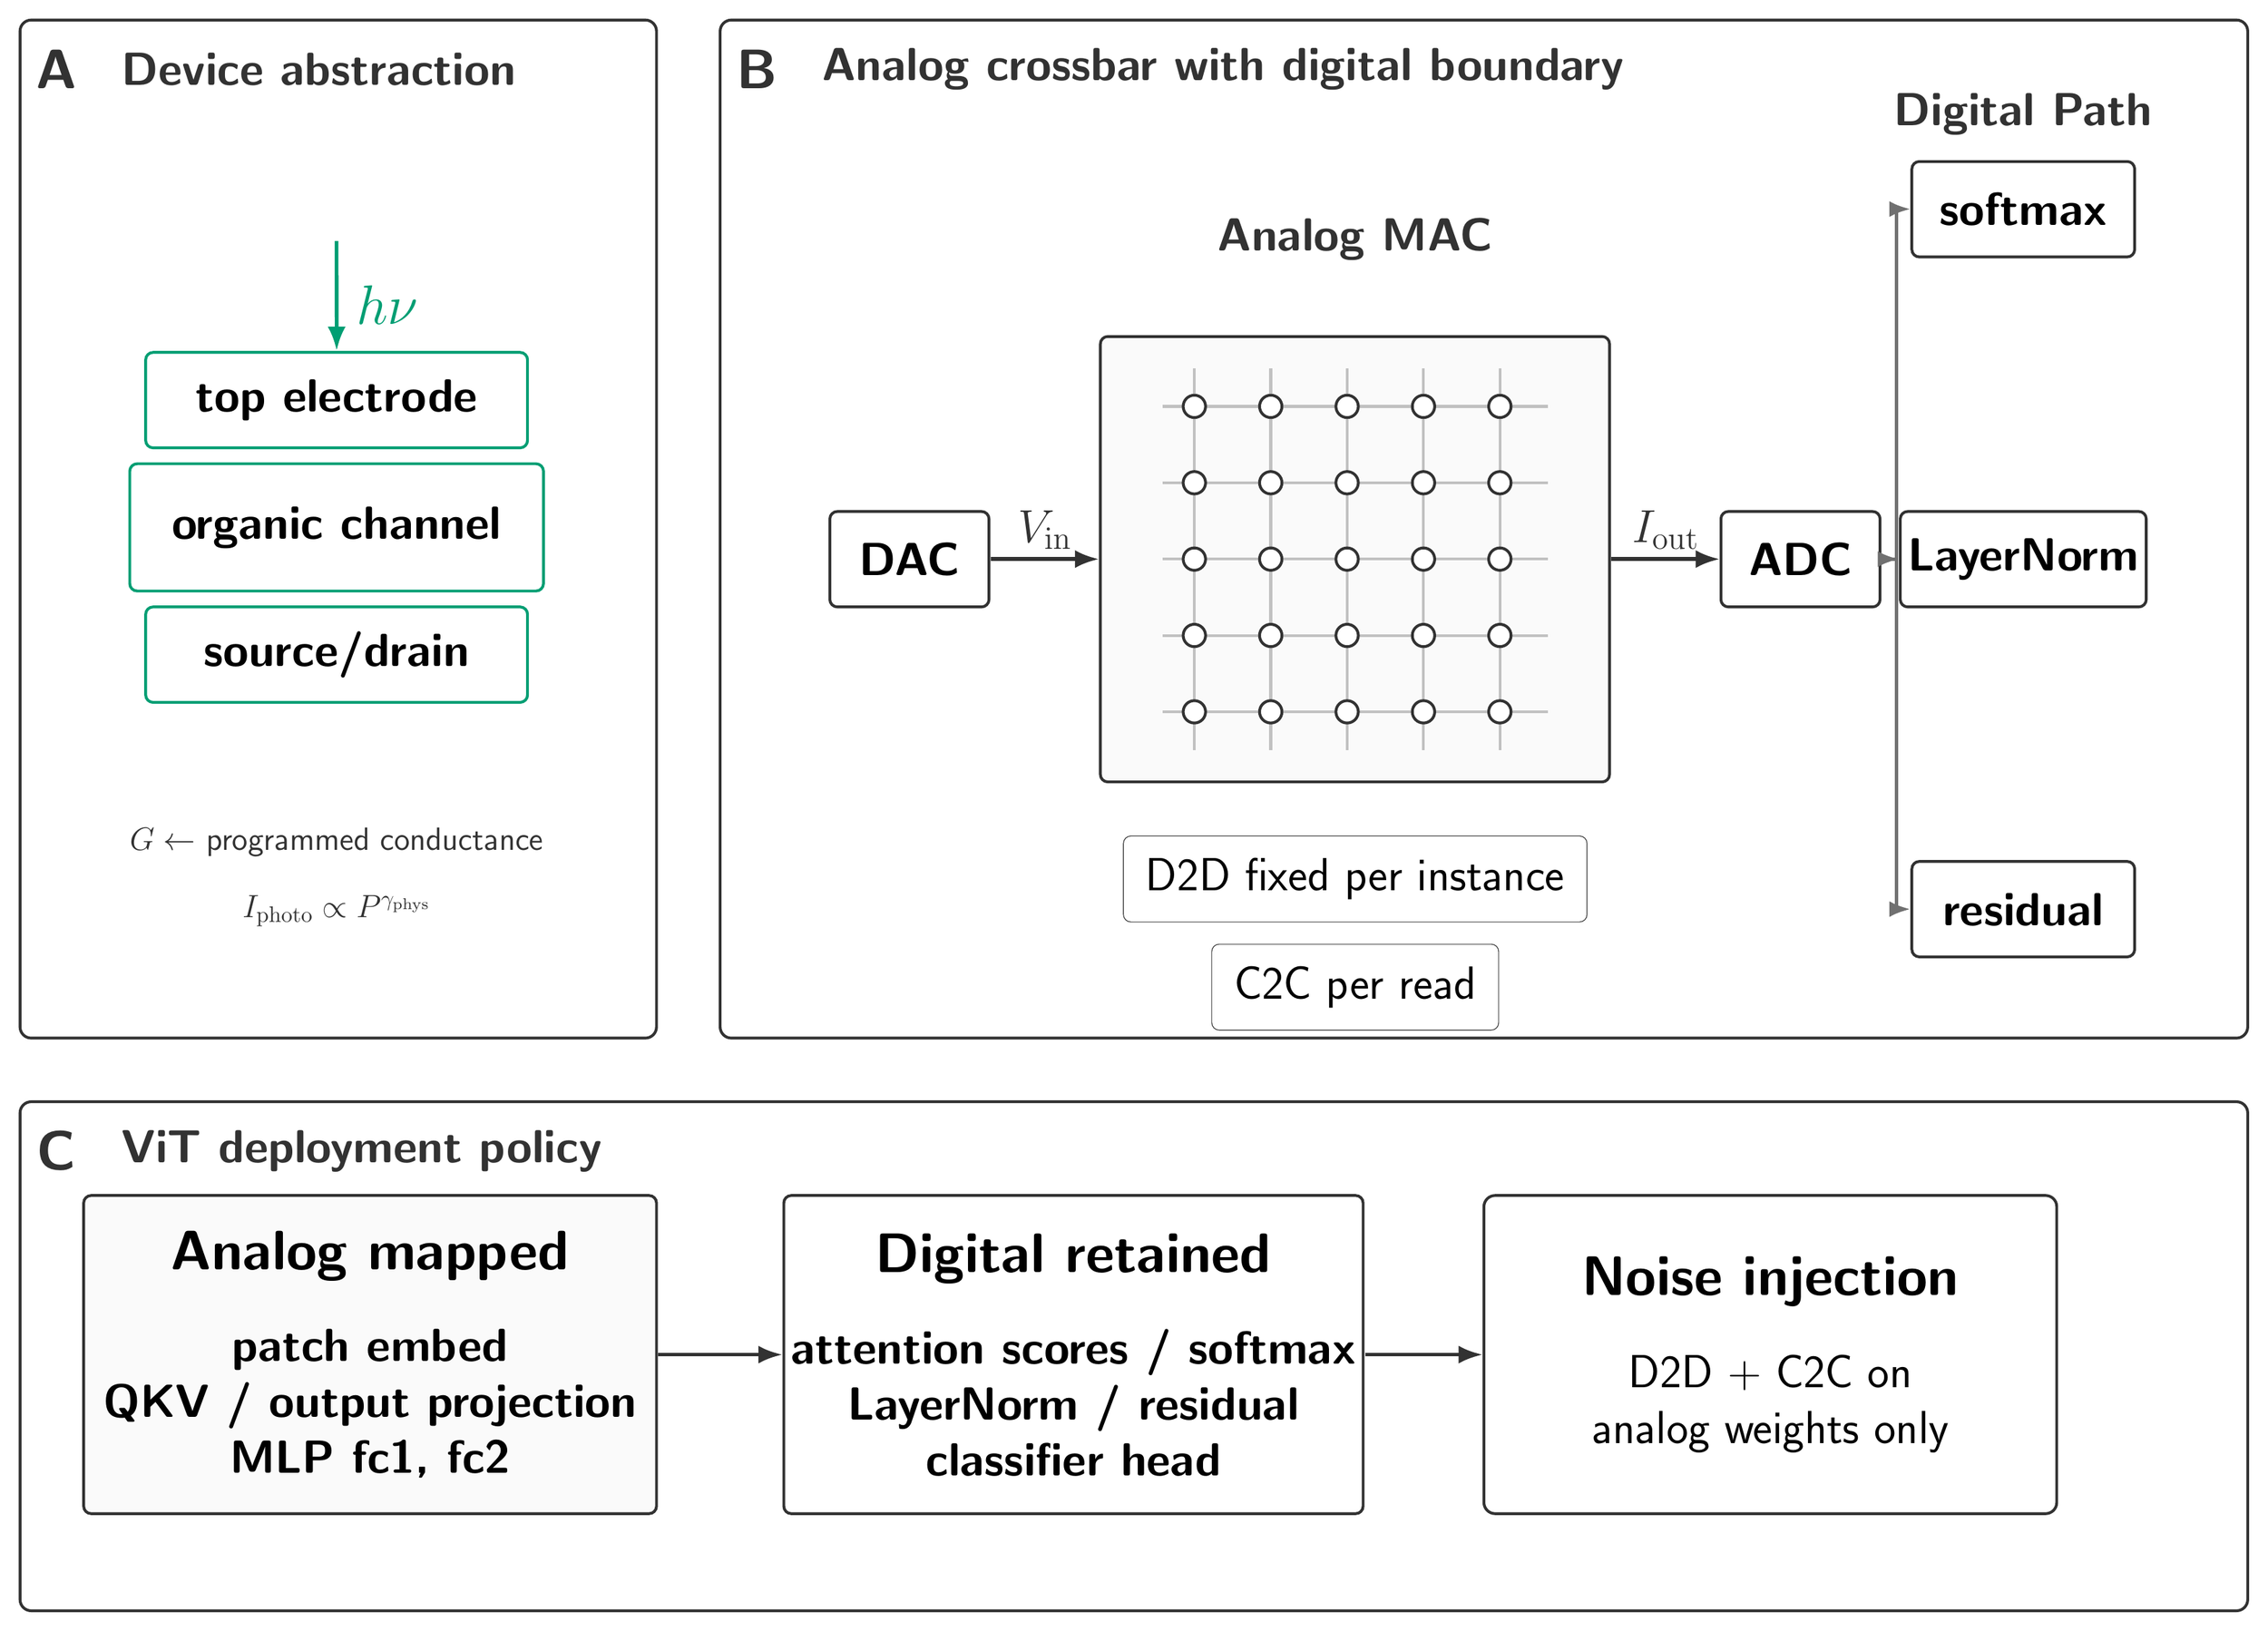
\begin{tikzpicture}[
  scale=1.2, transform shape,
  font=\sffamily,
  panel/.style={draw=lineColor, rounded corners=6pt, fill=white, line width=1.5pt},
  title/.style={font=\sffamily\bfseries\huge, text=lineColor, anchor=west},
  tag/.style={font=\sffamily\bfseries\Huge, text=lineColor},
  smalltext/.style={font=\sffamily\Large, text=lineColor, align=center},
  tinylabel/.style={font=\sffamily\huge, text=lineColor},
  analog/.style={draw=lineColor, fill=boxBg, rounded corners=4pt, line width=1.5pt, align=center, font=\huge\bfseries},
  digital/.style={draw=lineColor, fill=white, rounded corners=4pt, line width=1.5pt, align=center, font=\huge\bfseries},
  device/.style={draw=accentGreen, fill=white, rounded corners=4pt, line width=1.5pt, align=center, font=\huge\bfseries},
  arrow/.style={-{Latex[length=4.5mm]}, line width=2.0pt, draw=lineColor},
  softarrow/.style={-{Latex[length=4.0mm]}, line width=1.8pt, draw=lineColor!70}
]

% ------------------------------------------------------------------
% Panel A: device abstraction
% ------------------------------------------------------------------
\node[panel, minimum width=10.0cm, minimum height=16.0cm, anchor=north west] (pa) at (0,16.0) {};
\node[tag] at ($(pa.north west)+(0.6,-0.8)$) {A};
\node[title] at ($(pa.north west)+(1.5,-0.8)$) {Device abstraction};

\node[device, minimum width=6.0cm, minimum height=1.5cm] (top) at (5.0, 10.0) {top electrode};
\node[device, minimum width=6.5cm, minimum height=2.0cm] (semi) at (5.0, 8.0) {organic channel};
\node[device, minimum width=6.0cm, minimum height=1.5cm] (bot) at (5.0, 6.0) {source/drain};

\draw[arrow, accentGreen] (5.0, 12.5) -- (top.north);
\node[font=\sffamily\Huge\bfseries, text=accentGreen] at (5.8, 11.5) {$h\nu$};

\node[smalltext] at (5.0, 2.5) {$G \leftarrow$ programmed conductance\\[12pt]$I_{\mathrm{photo}} \propto P^{\gamma_{\mathrm{phys}}}$};

% ------------------------------------------------------------------
% Panel B: array + mixed-signal boundary
% ------------------------------------------------------------------
\node[panel, minimum width=24.0cm, minimum height=16.0cm, anchor=north west] (pb) at (11.0, 16.0) {};
\node[tag] at ($(pb.north west)+(0.6,-0.8)$) {B};
\node[title] at ($(pb.north west)+(1.5,-0.8)$) {Analog crossbar with digital boundary};

\node[digital, minimum width=2.5cm, minimum height=1.5cm] (dac) at (14.0, 7.5) {DAC};
\node[analog, minimum width=8.0cm, minimum height=7.0cm] (xb) at (21.0, 7.5) {};
\node[digital, minimum width=2.5cm, minimum height=1.5cm] (adc) at (28.0, 7.5) {ADC};

\draw[arrow] (dac.east) -- (xb.west) node[midway, above, tinylabel] {$V_{\mathrm{in}}$};
\draw[arrow] (xb.east) -- (adc.west) node[midway, above, tinylabel] {$I_{\mathrm{out}}$};

% Crossbar grid inside xb
\foreach \i in {0,...,4} {
  \draw[lineColor!30, line width=1.5pt] ($(xb.west)+(1.0, 2.4-1.2*\i)$) -- ($(xb.east)+(-1.0, 2.4-1.2*\i)$);
  \draw[lineColor!30, line width=1.5pt] ($(xb.west)+(1.5+1.2*\i, 3.0)$) -- ($(xb.west)+(1.5+1.2*\i, -3.0)$);
}
\foreach \i in {0,...,4} {
  \foreach \j in {0,...,4} {
    \node[circle, draw=lineColor, fill=white, minimum size=10pt, inner sep=0pt, line width=1.5pt] at ($(xb.west)+(1.5+1.2*\j, 2.4-1.2*\i)$) {};
  }
}

\node[font=\sffamily\huge\bfseries, text=lineColor] at ($(xb.north)+(0,1.5)$) {Analog MAC};
\node[draw=lineColor, fill=white, rounded corners=4pt, inner sep=10pt, font=\sffamily\huge] at ($(xb.south)+(0,-1.5)$) {D2D fixed per instance};
\node[draw=lineColor, fill=white, rounded corners=4pt, inner sep=10pt, font=\sffamily\huge] at ($(xb.south)+(0,-3.2)$) {C2C per read};

% Digital blocks on the right
\node[digital, minimum width=3.5cm, minimum height=1.5cm] (soft) at (31.5, 13.0) {softmax};
\node[digital, minimum width=3.5cm, minimum height=1.5cm] (norm) at (31.5, 7.5) {LayerNorm};
\node[digital, minimum width=3.5cm, minimum height=1.5cm] (res)  at (31.5, 2.0) {residual};

\coordinate (split) at (29.5, 7.5);
\draw[softarrow, -] (adc.east) -- (split);
\draw[softarrow] (split) |- (soft.west);
\draw[softarrow] (split) -- (norm.west);
\draw[softarrow] (split) |- (res.west);

\node[smalltext] at (31.5, 14.5) {\textbf{\huge Digital Path}};

% ------------------------------------------------------------------
% Panel C: deployment policy
% ------------------------------------------------------------------
\node[panel, minimum width=35.0cm, minimum height=8.0cm, anchor=north west] (pc) at (0, -1.0) {};
\node[tag] at ($(pc.north west)+(0.6,-0.8)$) {C};
\node[title] at ($(pc.north west)+(1.5,-0.8)$) {ViT deployment policy};

\node[analog, minimum width=9.0cm, minimum height=5.0cm, anchor=west] (ana) at (1.0, -5.0)
{\textbf{\Huge Analog mapped}\\[16pt] \huge patch embed\\QKV / output projection\\MLP fc1, fc2};

\node[digital, minimum width=9.0cm, minimum height=5.0cm, anchor=west] (dig) at (12.0, -5.0)
{\textbf{\Huge Digital retained}\\[16pt] \huge attention scores / softmax\\LayerNorm / residual\\classifier head};

\node[draw=lineColor, fill=white, rounded corners=6pt, minimum width=9.0cm, minimum height=5.0cm, align=center, font=\sffamily\huge, line width=1.5pt, anchor=west] (noise) at (23.0, -5.0)
{\textbf{\Huge Noise injection}\\[16pt] \huge D2D $+$ C2C on\\analog weights only};

\draw[arrow] (ana.east) -- (dig.west);
\draw[arrow] (dig.east) -- (noise.west);

\end{tikzpicture}
\end{document}
